\documentclass[12pt, titlepage, oneside]{article}
\usepackage[letterpaper, margin=1in]{geometry}
\usepackage{siunitx, booktabs, amsmath, enumitem, pdfpages, tabularx,caption, graphicx, pgfplots, textcomp}
\usepackage[siunitx]{circuitikz}
\sisetup{detect-weight=true, detect-family=true}
\usepackage{wrapfig}
\usepackage{mathrsfs}
\setlength\parindent{0pt}
\let\oldhat\hat
\let\oldvec\vec
\newcommand{\cross}{\bm{\times}}
\renewcommand{\hat}[1]{\oldhat{\mathbf{#1}}}
\usepackage{bm}
\renewcommand{\vec}[1]{\oldvec{\bm{#1}}}
\renewcommand{\hat}[1]{\oldhat{\bm{#1}}}
\renewcommand{\b}[1]{\textbf{#1}}


\begin{document}
	\section*{23.1: Properties of Electric Charges}
	
	Objects when they gain an excess or deficiency of electrons, they are said to become \textbf{charged}. There are two kinds of electrical charges which are named \textbf{positive} and \textbf{negative}. It is also important to note that electrically charged objects interact with other objects. 
	\vspace{2mm}
	
				\noindent\fbox{%
		\parbox{\textwidth}{%
		\textbf{Basic Properties of Charge}
		\begin{center}
			\textbf{Like charges Repel}
			
			\textbf{Opposite charges Attract}
		\end{center}
	}}	
	\vspace{2mm}
	
	Additionally, just like the law of conservation of mass, we have to consider the \textbf{conservation of charge}. The conservation of charge states the electric charge in a system is conserved in a closed system.
	\section*{23.3: Coulomb's Law}
	
	\noindent\fbox{%
		\parbox{\textwidth}{%
			\textbf{Coulomb's Law}
			\begin{align}
			F_e = k_e \dfrac{|q_1| |q_2|}{r^2}
			\end{align}
			$k_e = \SI{8.987e9}{Nm^2/C^2}$
			\begin{align}
			k_e = \frac{1}{4\pi \epsilon_0}
			\end{align}  
			$\epsilon_0 = \SI{8.8542 e-12}{C^2/N \cdot m^2}$
	}}	
	\vspace{1mm}

	The following equations above have two constants, $k_e$ and $\epsilon_0$. $k_e$ is \textbf{Coulomb's constant} which was determined empirically at first. $\epsilon_0$ is \textbf{permittivity of free space} which is the resistance of a vacuum to generate an electric field.
	
	The smallest unit of charge of free charge is the unit $e$ which can be used for protons or electrons.
	\vspace{2mm}
	
	\noindent\fbox{%
		\parbox{\textwidth}{%
			\textbf{Unit of Charge}
			
		
		\begin{equation}
		q_{electron} = (-1)e \hspace{2cm} q_{proton} = (+1)e
		\end{equation}
		$e = \SI{1.60218e-19}{C}$
	}}

	\vspace{1mm}
	The vectorial form describes the movement perfectly,
	\begin{equation*}
	\vec{F}_{12} = k_e \frac{q_1 q_2} {r^2}\,\hat{r}_{12}
	\end{equation*}
	In the equation above we describe the force experienced by $q_2$ because of $q_1$. $\hat{r}_{12}$ is a unit vector directed from $q_1$ to $q_2$. Drawing the following would help tremendously, remember the force acts on $q_2$ so it would only exist in $q_2$ FBD.
	
	\section*{23.4 Analysis Model: Particle in a Field}
	An electric field is said to exist in the region of space around a charged object which is called a \textbf{source charge}. A \textbf{test charge} is a small positive particle which is placed in a field to notice the electric field at that point. It should be noted that the test charge must be small enough such that it does not change the existing electric field.
	\vspace{1mm}
	
	An electric field vector is the force per charge for an arbitrary charge $q$ at a distance $r$,
	\vspace{2mm}
	
		\noindent\fbox{%
		\parbox{\textwidth}{%
			\textbf{Electric Field}
		\begin{equation}
		\vec{F} = q \vec{E}
		\end{equation}
		or
		\begin{equation}
		\vec{E} = k_e \frac{q}{r^2} \hat{r}
		\end{equation}
		$E = $N/C
	}}
	\vspace{2mm}
	
	Derived by placing a known test charge $q_0$ in the region of space about charge $q$,
	\begin{align*}
	\vec{F_e} = k_e \frac{q_0\,q}{r^2}\, \hat{r} 
	\end{align*}
	Dividing by our known test charge $q_0$,
	\begin{align*}
	\vec{E} = k_e \frac{q}{r^2}\, \hat{r} 
	\end{align*}
	\textbf{Notice}: The $\hat{r}$ points in the direction of the electric force on a \textbf{positive} test charge. 
	\begin{center}
	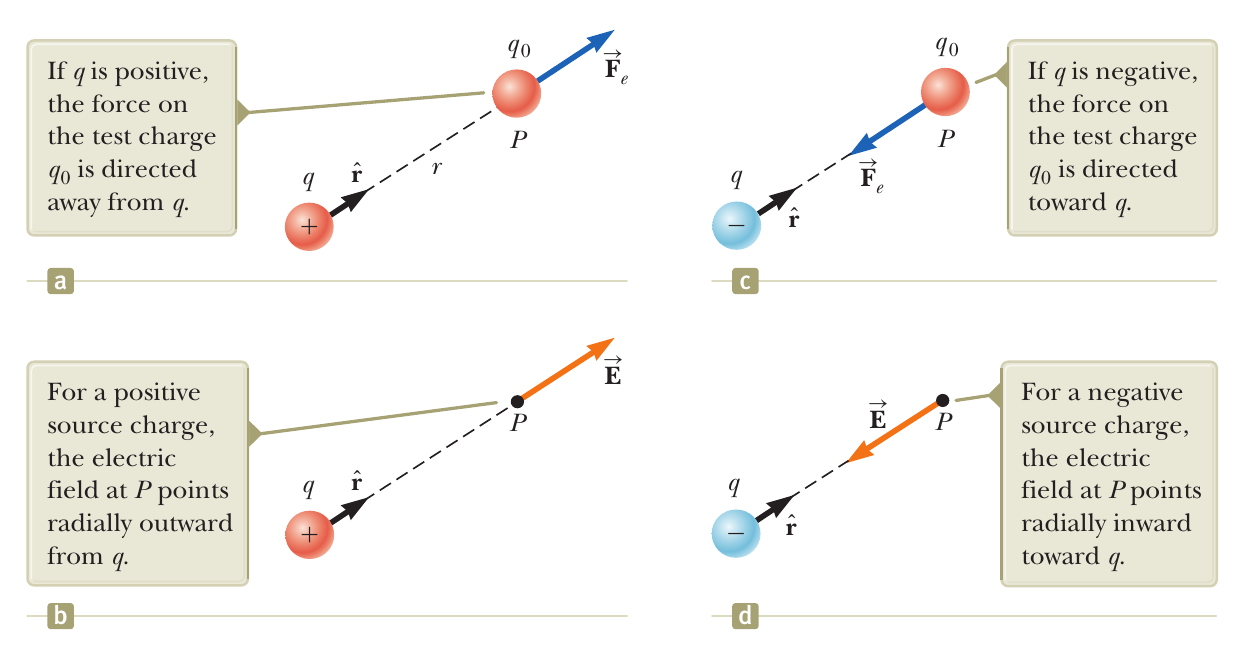
\includegraphics[scale=0.34]{1.png}
	\end{center}
	Since this is a vector quantity we can add the vectors,
	\begin{align*}
	\vec{E} = k_e \sum_i \,\dfrac{q_i}{r_i^2}\,\,\hat{r_i}
	\end{align*}
	This adds up all the charges and their respective distances from some point chosen.
	\section*{23.5 Electric Field of a Continuous Charge Distribution}
	\noindent\fbox{%
		\parbox{\textwidth}{%
		\textbf{Charge Densities For Uniform Materials}
		\begin{align}		
		\rho \equiv \frac{Q}{V}
		\end{align}	
		\textbf{Volume Charge Density} $\rho$, where $V$ is the \textbf{volume} and $Q$ is the \textbf{total charge}
				\begin{align}		
		\sigma \equiv \frac{Q}{A}
		\end{align}	
		\textbf{Surface Charge Density} $\sigma$, where $A$ is the \textbf{surface area} and $Q$ is the \textbf{total charge}
				\begin{align}		
		\lambda \equiv \frac{Q}{l}
		\end{align}	
		\textbf{Linear Charge Density} $\lambda$, where $l$ is the \textbf{length} and $Q$ is the \textbf{total charge}
		}}
	\vspace{1mm}
	
	This is not important now, but will become more applicable in Gauss' Law in a later unit.
	\section*{23.6 Electric Field Lines}
	
	Electric field lines are a great way to visualize the electric field,
	
	\begin{itemize}
	\item The electric field line $\vec{E}$ is perpendicular to the surface and has an arrow depicting the direction of $\vec{E}$.	
	\item The electric field density is the spacing of electrical field lines. This means when a surface has \textbf{uniform electric field}, this means everywhere on that surface the electric field lines which intersect perpendicular is proportional to the "density of the field"
	\item For positive charges, the field lines point outward. For negative charges, the field lines point inwards
\end{itemize}
\begin{center}
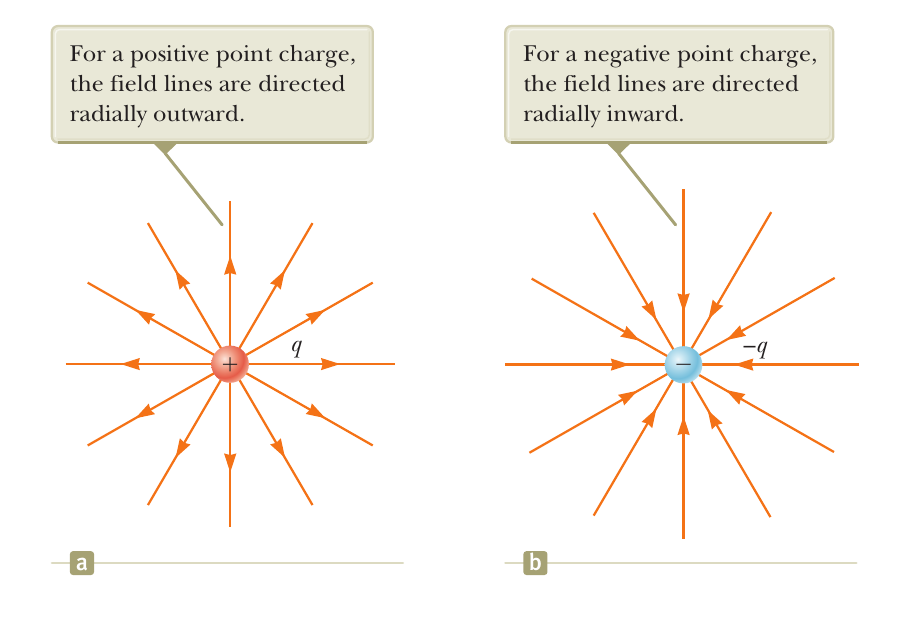
\includegraphics[scale=0.32]{2.png}
\end{center}
\textbf{Note}: There are areas where the electric fields of negative and positively charged fields cancel out, resulting in no field existing at that point in space. 
\begin{center}
	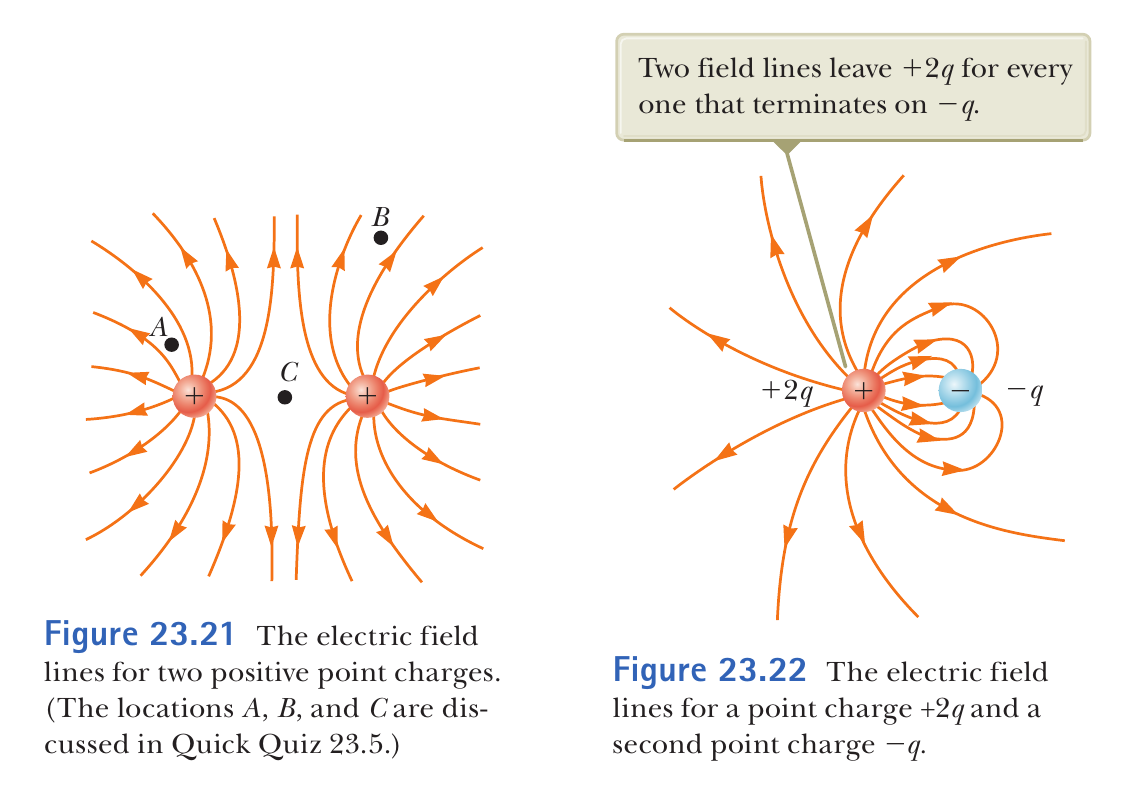
\includegraphics[scale=0.32]{3.png}
\end{center}
\section*{23.8 Motion of a Charged Particle in a Uniform Electric Field}
If there was a particle experiencing force due to a uniform electric field we can write,
\begin{align*}
\vec{F}_e = q \vec{E} = m\vec{a}
\end{align*}
Therefore, we can rearrange for acceleration,
\begin{align*}
\vec{a} = \frac{q\vec{E}}{m}
\end{align*}
This is only valid if $\vec{E}$ as the particle needs to move. Notice the similarities between this and gravity,
\begin{align*}
\vec{F}_g = \vec{g}m = m\vec{a}
\end{align*}
Assuming the particle was close to the ground, therefore experiencing a nearly uniform gravitational field,
\begin{align*}
\vec{a} = \frac{m \vec{g}}{m} = \vec{g}
\end{align*}
\end{document}